\section{Challenges}
In previous sections of large scale circuit implementation, there are a few challenges, but all boils down to non ideal opamp behaviour. The non ideality characteristics arise in every practical devices, but the opamp implemented before has worse condition. This is especially the case when the internal circuit design of a LM741 opamp (Figure \ref{fig:opampint}) is obtained from Texas Instrument but implemented using TSMC 65nm process design kit (PDK). High precision opamp design are proprietary and therefore not available on the manufacturer's website.
\label{sect:cha}
\begin{figure}[h]
	\centering
	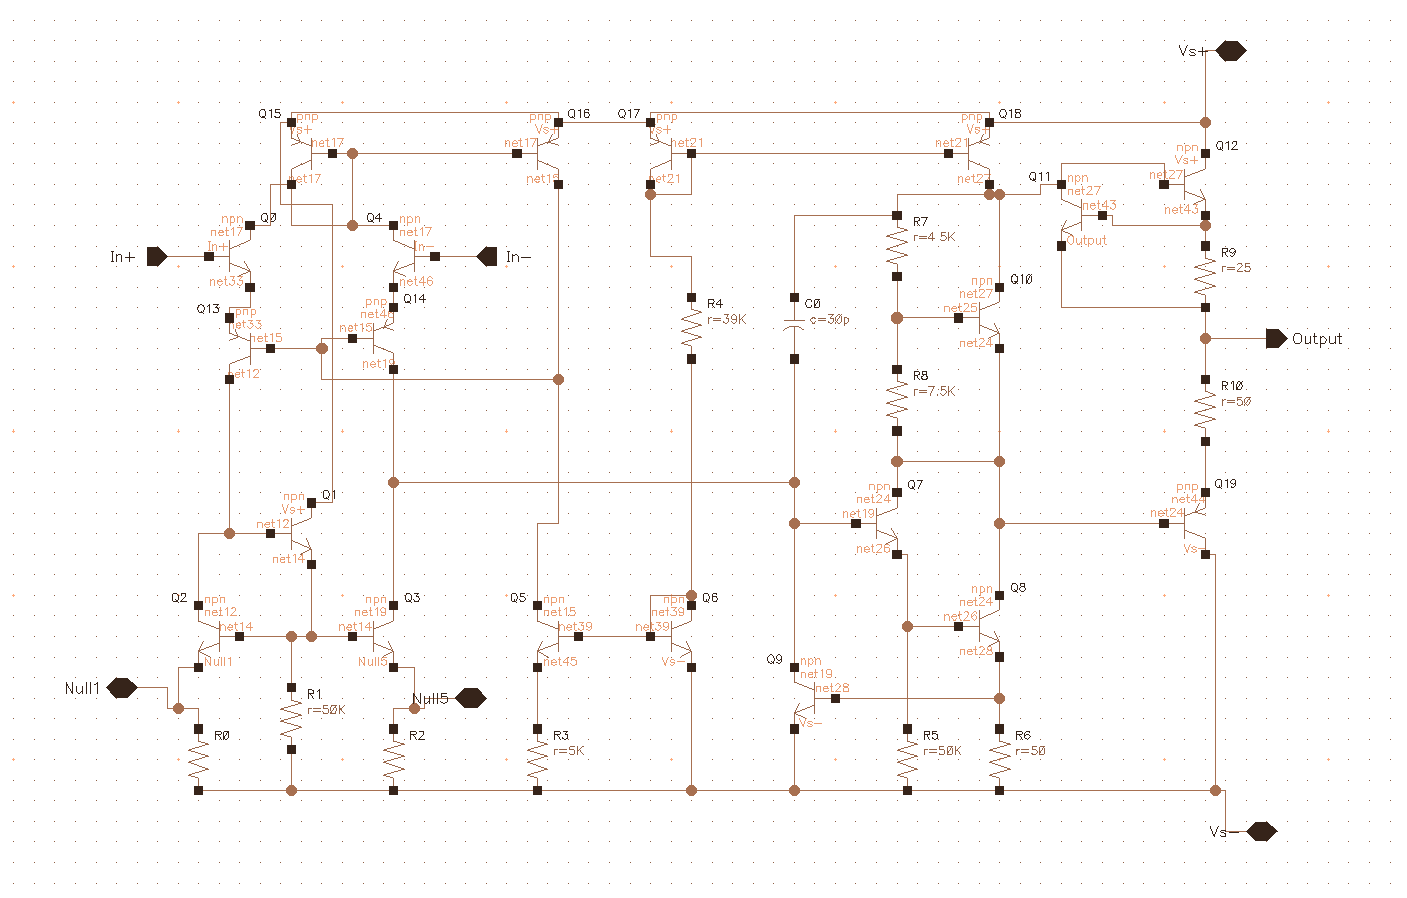
\includegraphics[scale=0.35]{opamp.png}
	\caption{Internal circuitry of TI LM741 operational amplifier (OpAmp)}
	\label{fig:opampint}
\end{figure}
The model provided us with 2 null input pins to calibrate opamp performance if there are device mismatches (transistor pairs from different vendor, collector and emitter resistors, etc.) due to manufacturing imperfection. In a non ideal case in Figure \ref{fig:opampchar}, if $V_+ = V_- = 0$, $V_o = 0$. However, with mismatches, there is a finite $V_o$. In Figure \ref{fig:opampnullset}, we can add resistors in parallel with $R_0$ and $R_2$ as shwon in Figure \ref{fig:opampint}. These resistors are adjustable, together known as potentiometer as $R_0$ and $R_1$ in Figure \ref{fig:opampnullset} add up to a fixed resistance. If adjustment is successful, we get $V_o = 0$ as needed. However, this is not the case. It doesn't matter if we swap out the potentiometer for 2 independent resistor, it still does not work as it makes only tiny difference to the output.
\begin{figure}[h]
	\centering
	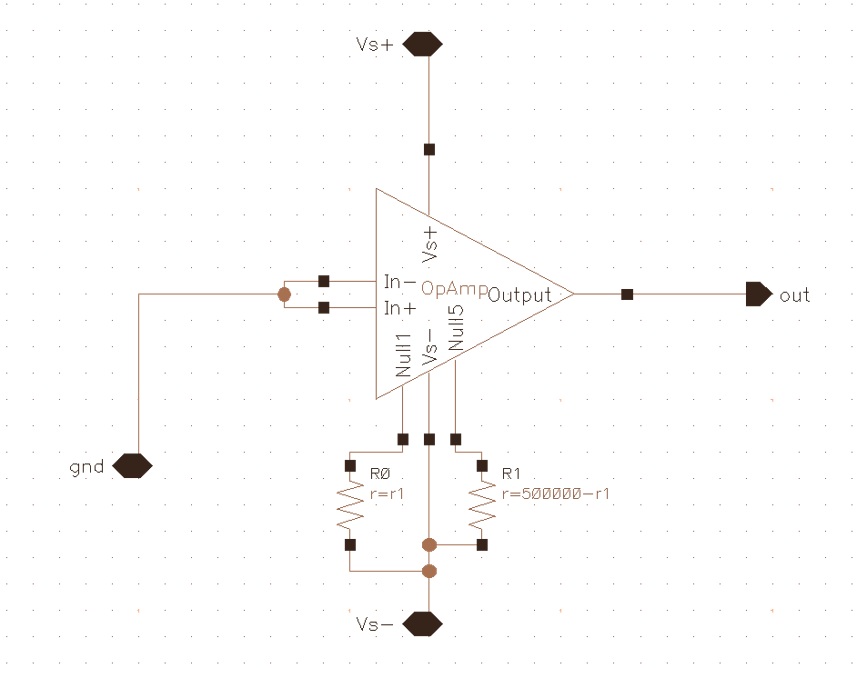
\includegraphics[scale=0.35]{opampnull.png}
	\caption{TI LM741 OpAmp null offset}
	\label{fig:opampnullset}
\end{figure}
Figure \ref{fig:parallelr} show the effective resistance we can achieve if we keep adding resistance in parallel with $R_0$ and $R_2$ in Figure \ref{fig:opampint}. We observe that the limit of $1k\Omega$ (resistance of $R_0$ and $R_2$ where $R_0=R_2=1k\Omega$) is reached when parallel resistance tends to infinity.

The formula for the graph plot is:
$$R_{\text{effective}} = \frac{R_{//}\times R}{ R_{//}+R}$$
\begin{figure}[H]
	\centering
	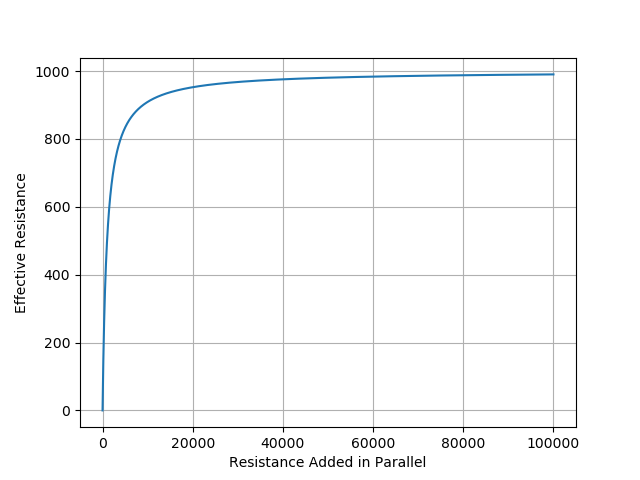
\includegraphics[scale=0.7]{parallelr.png}
	\caption{Graph of effective resistance vs resistance added in parallel with existing resistance $R=1\text{k\Omega}$}
	\label{fig:parallelr}
\end{figure}
Out-of-the-box thinking was required for opamp to work. Hence, both 2 null input pins were removed and the 2 $1k\Omega$ resistors in Figure \ref{fig:opampint} were tuned independently and it worked. The final resistance setting for those 2 resistors are $1k\Omega$ and $1.138M\Omega$ for left and right resistors respectively.

In Figure \ref{fig:opamptune}, we want to identify optimal operation condition of opamp with minimal error. Initially, we fixed $R_0=R_1$ as shown in Figure \ref{fig:opampnonideal} as increased their value in tandem. In an ideal opamp summing application, a single $V_{\text{in}}$ should yield $V_{\text{in}} = -V_o$. It works as expected for $R_1=50k\Omega$,$R_0=50k\Omega$ and $R_1=500k\Omega$,$R_0=500k\Omega$ where $V_o$ decreases linearly until it reaches $-V_{\text{sat}}$. However, opamp exhibits erratic behaviour for $R_1=2k\Omega$,$R_0=2k\Omega$ where $V_o$ decreases initially before rising again unpredictably. This is suspected as caused by high power consumption. Using $\frac{{V_{\text{in}}}^2}{R}$ and assume virtual ground at $0V$, for the same $V_{\text{in}}$, taking $\frac{{V_{\text{in}}}^2}{2k}$ as reference, for $R_1=50k$, the power is reduced by 25 times, and for $R_1=500k$, the power is further reduced by 10 times.
\begin{figure}[H]
	\centering
	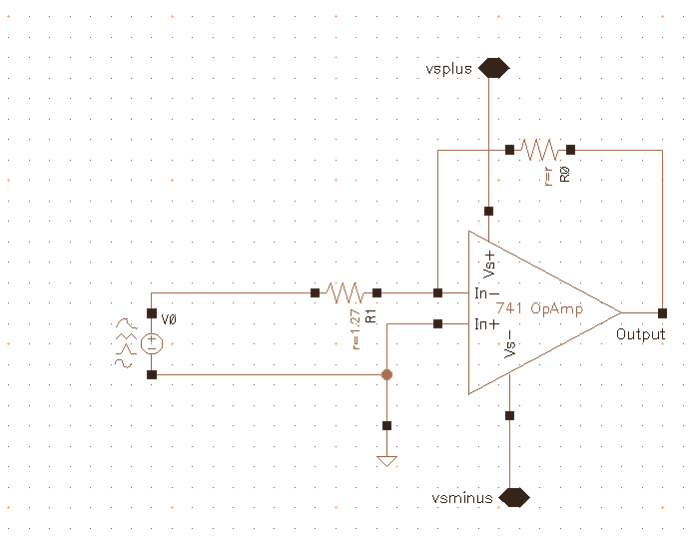
\includegraphics[scale=0.5]{opamptune.png}
	\caption{Tuning output resistance $R_F$ ($R_0$) for input resistance ($R_1$) between $1\text{k\Omega}$ and $3\text{k\Omega}$}
	\label{fig:opamptune}
\end{figure}
\begin{figure}[H]
	\subfloat[virtual ground voltage with different resistor pair
	]{
		\centering
		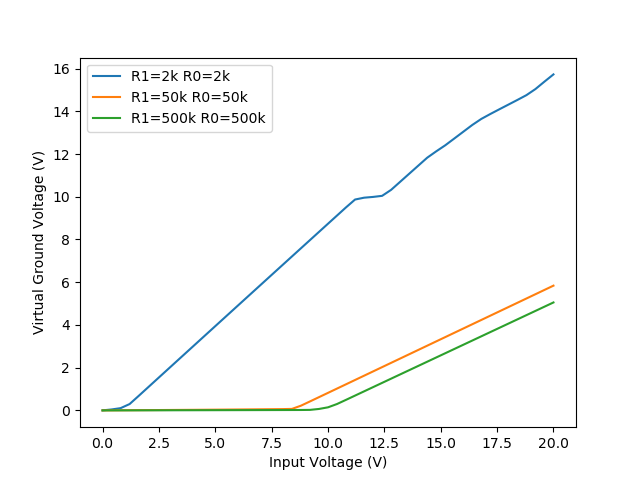
\includegraphics[scale=0.5]{virgnd.png}
	}
	\subfloat[Output voltage with different resistor pair]{
		\centering
		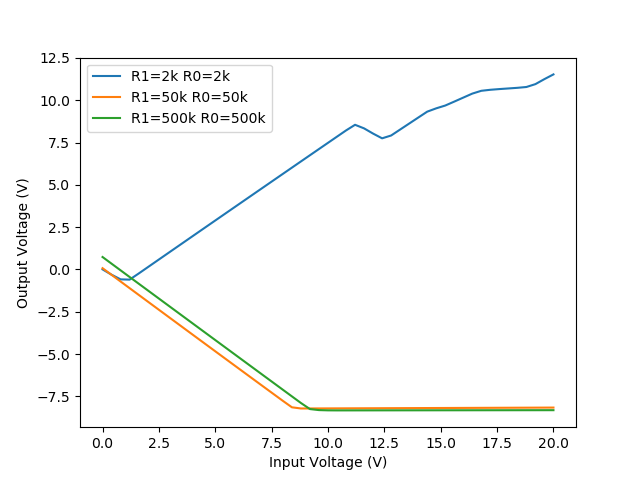
\includegraphics[scale=0.5]{vout.png}	
	}
	\caption{Non ideal opamp characteristic (based on Figure \ref{fig:opamptune})}
	\label{fig:opampnonideal}
\end{figure}
For virtual ground voltage, ideally, we expect the voltage to be $0V$ regardless since it is a critical condition for our computation. However, this condition is not met for the high power case ($R_1=2k\Omega$,$R_0=2k\Omega$). The virtual ground voltage is low initially and when $V_{\text{in}}$ increases, virtual ground condition breaks and its voltage increases too.

Table \ref{tbl:riv} follows that of Figure \ref{fig:opamptune}, where different value for $R_1$ and $R_0$($R_F$) were tested. Range of $R_1$ is between $1k\Omega$ to $3k\Omega$ and hence only these 2 extreme values of $R_1$ are examined with different $R_F$ values to find out the optimal setting through varying $V_{\text{in}}$. The best case is having the lowest value for $V_{\text{virtual gnd,min}}$ and $V_{\text{virtual gnd,max}}$ to closely approximate virtual ground condition. When $R_1=1k\Omega$, the optimal $R_F$ is almost indiscernible. One notable phenomenon in this table is higher $V_{\text{virtual gnd,max}}$ corresponds to lowest $I_{\text{in,max}}$ and therefore lowest $I_{\text{out,max}}$ due to reduced potential difference between $V_{\text{in}}$ and $V_{\text{virtual gnd}}$.

A way to calibrate $V_{\text{virtual gnd}}$ has been discovered though adjusting $+V_{\text{sat}}$ and $-V_{\text{sat}}$. This is possible due to the effect of Voltage Divider Rule.

In a voltage divider rule, $V_{\text{virtual gnd}}$ is determined by:
$$V_{\text{virtual gnd}}=\frac{\frac{+V_{\text{sat}}}{R_0}+\frac{-V_{\text{sat}}}{R_1}}{\frac{1}{R_0}+\frac{1}{R_1}}$$
In a case with 2 $V_{\text{in}}$, $V_{\text{virtual gnd}}$ becomes:
$$V_{\text{virtual gnd}}=\frac{\frac{+V_{\text{sat}}}{R_0}+\frac{-V_{\text{sat}}}{R_3}+\frac{V_1}{R_1}+\frac{V_2}{R_2}}{\frac{1}{R_0}+\frac{1}{R_3}+\frac{1}{R_1}+\frac{1}{R_2}}$$
We can expected many more $V_{\text{in}}$ for a larger scale circuit. Since we can cannot tune individually the resistors, we stick to tuning $\pm V_{\text{sat}}$. However, in a very large scale circuit where we have many terms, tuning 1 or 2 terms has insignificant effect, which explains why we have huge, similar $S.D.$ error for large scale $\text{3}^{\text{rd}}$ version and $\text{4}^{\text{th}}$ dual stage version neuromorphic circuit.

All these suboptimal performance (i.e. non-zero $V_{\text{virtual gnd}}$ and low output current) leads to poor gain. To counter this effect, different resistor pertaining to opamp scaling (not resistor array linked to weights) are tuned.

Concretely, Equation \ref{eq:final34compdecomp} is modified to the form:
$$V_{\text{out}}=R_{Fo2}\left(\frac{R_{Fo1}}{R_{Fi}} \left(\frac{1}{\left| R_F\right|r_1}V_1+\frac{1}{\left| R_F\right|r_2}V_2+... \right)-\left(\frac{1}{R_{aFi}}V_1+\frac{1}{R_{aFi}}V_2+... \right)\right)$$
where $R_{aFi}=\frac{1000s}{w_{c,8}}$, $R_{Fi}=1000s$ , $R_{Fo2}=\frac{1000s}{w_{c,0}-w_{c,8}}$  and $s$ is a scale factor to scale the summing neuron output to ideal value.
\begin{figure}[H]
	\centering
	\subfloat[Virtual ground voltage]{
		\centering
		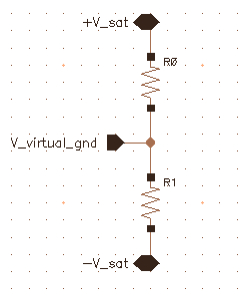
\includegraphics[scale=0.5,valign=t]{vgnd.png}
	}
	\subfloat[Virtual ground voltage with many $V_{\text{in}}$]{
		\centering
		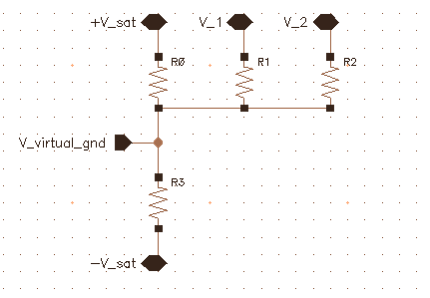
\includegraphics[scale=0.5,valign=t]{vgndmany.png}
	}
	\caption{Voltage Divider Rule}
	\label{fig:vgnd}
\end{figure}
Simulation time is also one of the challenges. Simulation time grow proportionally with network size. There are 10000 test samples in our MNIST test data set (See Case Study Section). For a network size of 10 by 20, the simulation time foreach sample take about 1 second. However, for the same test dataset with a network size of 20 by 784, the simulation time for a sample takes around $2\frac{1}{2}$ hours. So, to tune a parameter and to see its result before proceeding to the next adjustment of the same parameter is very time consuming, not to mention tuning for all other parameters. It is mostly a waiting game. The parameters tuned for a small network is also incompatible for a larger network due to practical non ideality.
\begin{table}[H] 
	\centering
	\subfloat[$R_1=1\text{k\Omega}$]{
\begin{tabular}[t]{cccccccc}
	\hline
	$R_F(\text{k\Omega})$ & $I_{\text{in,min}}(\text{A})$ & $I_{\text{in,max}}(\text{A})$ & $I_{\text{out,min}}(\text{A})$ & $I_{\text{out,max}}(\text{A})$ & $V_{\text{virtual gnd,min}}(\text{V})$ & $V_{\text{virtual gnd,max}}(\text{V})$\\ 
	\hline
	\hline
	1 & -730.89n & 313.18u & -2.2189u & 310.71u & 730.9u & 86.86m\\ 
	2 & -727.74n & 312.09u & -2.2157u & 309.61u & 727.7u & 87.91m\\ 
	4 & -721.438n & 309.897u & -2.2093u & 307.4u & 721.4u & 90.1m\\ 
	8 & -708.83n & 305.39u & -2.1965u & 302.85u & 708.8u & 94.61m\\ 
	16 & -684.22n & 295.73u & -2.1716u & 293.14u & 684.2u & 104.3m\\ 
	32 & -636.65n & 261.518u & -2.12332u & 258.761u & 636.7u & 138.5m\\ 
	64 & -541.745n & 135.729u & -2.03317u & 132.789u & 547.7u & 264.3m\\ 
	128 & -391.155n & 70.1832u & -1.87439u & 67.2269u & 392.1u & 329.8m\\ 
	256 & -142.562n & 36.8194u & -1.62232u & 33.8592u & 142.6u & 363.2m\\ 
	512 & -194.7n & 19.971u & -1.2803u & 17.009u & -197.4u & 380.0m\\ 
	1024 & 566.9n & 11.495u & -902.95n & 8.5331u & -566.9u & 388.5m\\
	\hline
\end{tabular}}
	\qquad
	\subfloat[$R_1=3\text{k\Omega}$]{
	\begin{tabular}[t]{cccccccc}
	\hline
	$R_F(\text{k\Omega})$ & $I_{\text{in,min}}(\text{A})$ & $I_{\text{in,max}}(\text{A})$ & $I_{\text{out,min}}(\text{A})$ & $I_{\text{out,max}}(\text{A})$ & $V_{\text{virtual gnd,min}}(\text{V})$ & $V_{\text{virtual gnd,max}}(\text{V})$\\ 
	\hline
	\hline
	1 & -257.14n & 362.95u & -1.7457u & 360.31u & 771.4u & 111.2m\\ 
	2 & -256.26n & 362.14u & -1.7448u & 359.49u & 768.8u & 113.6m\\ 
	4 & -254.47n & 360.45u & -1.7429n & 357.78u & 763.4u & 118.6m\\ 
	8 & -251.21n & 356.71u & -1.7395u & 353.98u & 753.6u & 129.9m\\ 
	16 & -244.09n & 347.28u & -1.7321u & 344.46u & 732.2u & 158.2m\\ 
	32 & -230.374n & 236.374u & -1.7178u & 233.866u & 691.1u & 90.88m\\ 
	\rowcolor{lg} 64 & -203.673n & 117.933u & -1.68998u & 115.848u & 611.0u & 46.2m\\ 
	128 & -152.904n & 69.0335u & -1.63708u & 66.15u & 458.7u & 192.9m\\ 
	256 & -60.6307n & 36.5236u & -1.54094u & 33.5749u & 181.9u & 290.4m\\ 
	512 & 94.008n & 19.889u & -1.3798u & 16.931u & -282.0u & 340.3m\\ 
	1024 & 321.43n & 11.471u & -1.1429u & 8.5107u & -964.3u & 365.6m\\
	\hline
\end{tabular}}
	\caption{Table of $R_1$, current $I_{\text{in}}$ flowing from $R_1$ into virtual ground , current $I_{\text{out}}$ flowing from virtual ground into $R_F$ and voltage $V_{\text{virtual gnd}}$ of virtual ground (Optimal performance is highlighted in green)}
	\label{tbl:riv}
\end{table}